% !TEX root = dokumentation.tex
\section{Implementierung}\label{sec:impl}
In diesem Kapitel wird die konkrete Entwicklung des Spieles beschrieben. Dabei werden sowohl die verschiedenen Prototypen betrachtet, wichtige Design-Entscheidungen offen gelegt und die technischen Hintergründe erläutert.
\subsection{Prototyping}
	Als Basis der Implementierung wird eine in Unity vorhandene Vorlage verwendet,\footnote{Zu finden unter \url{https://www.assetstore.unity3d.com/en/\#!/content/32351} (abgerufen am 2017.05.14)} welche im Lauf der Entwicklung entsprechend angepasst und erweitert wird. Zu dieser Vorlage gehören ein vereinfachtes Modell eines Autos, eine Kamera, welche sich hinter dem Fahrzeug befindet und eine einfache Nutzersteuerung für die Tastatur.

	In diesem Abschnitt der Studienarbeit sollen nun die Prototypen in chronologischer Reihenfolge dargestellt werden, um die Entwicklung des Spiels zu verdeutlichen. Alle Stadien des Spiels werden sowohl von den Entwicklern, wie auch ausgewählten Testspielern geprüft. Das erhaltene Feedback bietet somit die maßgebliche Grundlage für die Änderungen zwischen zwei Prototypen. Eine ausführliche Darlegung der Design-Entscheidungen befindet sich im folgenden Kapitel.
	\begin{enumerate}[itemindent=*,label=\textbf{Prototyp \arabic*}]
		\item{ Für den Beginn der Entwicklung wird zunächst eine Kopie der genannten Vorlage angefertigt. Auf Basis der grundsätzlichen Spielidee wird die Kamera oberhalb des Fahrzeugs positioniert, um eine Top-Down Ansicht zu erhalten. Die hinter dem Fahrzeug positionierte Kamera rotiert bei einer Drehung mit dem Fahrzeug, um die Blickrichtung mit der Fahrtrichtung gleichzusetzen. Dieses Drehverhalten bleibt bei einer Umpositionierung der Kamera in eine Top-Down Ansicht erhalten. Zwecks besserer Übersichtlichkeit wird dieses Drehverhalten unterbunden und die Kamera lediglich relativ zur Position, jedoch nicht der Rotation des Fahrzeugs erweitert. Um das Spiel auf mobilen Endgeräten spielen zu können, ist eine zunächst vereinfachte Steuerung über einen Joystick und zwei Buttons, vorwärts und rückwärts, nötig. Die Eingaben des Joysticks werden relativ zur Rotation des Fahrzeugs verarbeitet, somit führt beispielsweise ein \enquote{nach links ziehen} des Joysticks dazu, dass das Fahrzeug eine Linkskurve fährt. Die vertikale Achse des Joysticks findet in diesem Prototyp keine Verwendung. }
		\item{ Für den zweiten Prototyp steht die Weiterentwicklung der Steuerung im Fokus. Für eine neue Umsetzung der Steuerung werden sowohl die horizontale, wie auch die vertikale Achse benötigt. Anschließend wird die Steuerung nicht relativ zur Ausrichtung des Fahrzeugs, sondern relativ zur Blickrichtung der Kamera implementiert. Somit schlägt das Fahrzeug immer die gleiche Richtung ein, wie der Joystick abhängig von seinem Mittelpunkt bewegt wird. Ein Ziehen des Joysticks nach rechts führt somit in jedem Fall dazu, dass das Fahrzeug nach rechts fährt. Die vorherige Fahrtrichtung des Fahrzeugs spielt dabei keine Rolle. }
		\item{ Auch der dritte Prototyp des Spiels hat die grundsätzliche Steuerung zum Ziel. Auf Basis mehrerer erhaltenen Kritiken soll das Verhalten des \enquote{Rückwärts-Pedals} verändert werden. Hauptkritikpunkt in diesem Fall ist, dass ein reales Fahrzeug kein eigens Pedal für den Rückwärtsgang besitzt. Mit einer Veränderung dieses Steuerungselements verändert sich das Rückwärts-Pedal zu einem Bremspedal. Ein Betätigen dieser Schaltfläche reduziert die Fahrtgeschwindigkeit bis zum Stillstand. Dem somit fehlenden Rückwärtsgang wird zunächst keine Beachtung geschenkt, dies soll mit einem späteren Prototyp implementiert werden.}
		\item{ Um die Optik des Spiels aufzuwerten, steht für den vierten Prototyp die Benutzeroberfläche im Fokus. Dabei werden sowohl für alle Buttons, wie auch für den Joystick eigene Grafiken erstellt. Alle Grafiken der Benutzeroberfläche folgen dem gleichen Konzept und vermitteln somit ein einheitliches Gesamtbild. Für die Gestaltung der Buttons für Gas und Bremse wird eine Evaluation durchgeführt. Der vorläufige Gewinner dieser Evaluation sind zwei Tachos, wobei ein Tacho einen hohen Wert und ein Tacho einen niedrigen Wert anzeigt. }
		\item{ Mit dem fünften Prototyp kann der Rückwärtsgang implementiert werden. Ein \enquote{nach Hinten ziehen} des Joysticks führt dabei zu einer Änderung der Fahrtrichtung des Fahrzeugs. Bei Betätigung des Gaspedals fährt das Fahrzeug somit rückwärts. Auch die Steuerung wird in diesem Fall so invertiert, dass das Fahrzeug weiterhin der Ausrichtung des Joysticks folgt. Weiterhin wird bei der Entwicklung dieses Prototyps ein Anzeigen der Aufgaben ermöglicht. Das Durchfahren eines Auslösers führt dazu, dass auf dem Bildschirm eine zufällige Aufgabe aus der Liste aller möglichen Aufgaben gewählt wird. Die möglichen Lösungen dieser Aufgabe werden zu diesem Zeitpunkt noch nicht angezeigt. Zusätzlich zu den Änderungen an der Spielmechanik existiert seit diesem Prototyp eine Minimap, welche dem Spieler den kommenden Streckenverlauf transparent auf dem Bildschirm anzeigt. }
		\item{ Die Finalisierung der Aufgaben innerhalb der Level ist der Kernaspekt des sechsten Prototyps. Dabei werden zunächst neben der Aufgabe auch zwei mögliche Lösungen dieser Aufgabe angezeigt. Die Lösungen der Aufgaben sind entweder in Blau oder in Rot eingefärbt, welche Farbe für die richtige Lösung verwendet wird, ist dabei zufällig gewählt. In den einzelnen Rennen werden den existierenden Weggabelungen Pfeile hinzugefügt, welche in den Farben der Aufgaben eingefärbt sind. Somit sieht der Spieler unmittelbar, welcher Weg zu welcher möglichen Lösung gehört. In jedem möglichen Weg befindet sich ein weiterer Auslöser, welcher die Auswertung der Aufgaben anstößt. Dabei ist mit jedem Auslöser eine der möglichen Antworten assoziiert. Somit kann überprüft werden, ob die Aufgabe korrekt gelöst ist. }
		\item{ Die siebte Version des Spiels stellt die Fertigstellung der Fahrzeugsteuerung dar. Der Wechsel zwischen dem Vorwärtsgang und dem Rückwärtsgang soll nur möglich sein, wenn das Fahrzeug still steht. Durch diese Änderung führt ein \enquote{Verreißen} des Joysticks lediglich zu einer Richtungsänderung, jedoch nicht mehr zum abrupten Abbremsen des Fahrzeugs. Da die generelle Steuerung als \enquote{zu empfindlich} kritisiert wird, wird eine Lenkungsverzögerung implementiert. An diesem Punkt erreicht die Steuerung den finalen Status.}
		\item{ Um ein Schließen der App ohne Datenverlust zu gewährleisten, wird eine Speicherung des Spielstands implementiert. In diesem Spielstand ist gespeichert, welche Rennen ein Nutzer bereits abgeschlossen hat, welche Pokalrennen bereits freigespielt sind, wie viele Münzen der Spieler besitzt und wie viele Aufgaben bereits erfolgreich gelöst sind. Eine Statistik, die den Lernerfolg über die Anzahl der gelösten Aufgaben darstellt, ist möglich, wird jedoch im Rahmen der Studienarbeit nicht realisiert. Weiterhin erhalten die einzelnen Rennen eine Auswertung darüber, ob das Rennen gewonnen ist. Die genauen Kriterien für das Gewinnen eines Rennens befinden sich im folgenden Kapitel. Durch die nun verfügbaren Informationen über die Anzahl an Münzen ist die Einführung des Ingame-Shops möglich. Dieser ist als eigenes Level realisiert und über Startmenü des Spiels erreichbar.}
		\item{ Damit das Spiel auch multilingual nutzbar ist, sollen jegliche Texte durch Symbole ersetzt werden. Weitere Symbole, welche dem gleichen Konzept wie bisherige Buttons folgen werden entworfen und umgesetzt. Mit dem Einbau dieser Symbole im Spiel sind jegliche Texte im Spiel nicht mehr nötig. Somit ist das Spiel grundsätzlich universal einsetzbar, die Sprache der Spieler ist irrelevant. Um die Dynamik und das Spielgefühl zu verbessern, werden dem Spiel verschiedene Töne hinzugefügt. So wird beispielsweise ein korrektes Lösen einer Aufgabe mit Jubel belohnt. Eine Kollision mit Objekten der Karte verursacht nun ebenso Geräusche. Zusätzlich erhält das Spiel Hintergrundtöne, welche die Spielwelt lebendiger wirken lassen. Mit der Fertigstellung dieses Prototyps ist die gewünschte Grundfunktionalität erreicht. Alle weiteren Schritte in der Entwicklung führen zu weiteren Levelpacks und spielbaren Leveln.}
	\end{enumerate}
\subsection{Design-Entscheidungen in der Entwicklung}
In diesem Kapitel sollen während des Prototypings aufgetretene Designentscheidungen aufgegriffen und erläutert werden. Dabei werden die Argumente sowie Meinungen von Testspielern einbezogen.
	\subsubsection{Automatische Beschleunigung Vs. Gaspedal}
	Kern dieser Entscheidung ist die Frage, ob der Nutzer einen Button betätigen muss, damit sein Fahrzeug fährt. Als automatisches Gas sind hierbei zwei Interpretationen möglich:
	\begin{itemize}
	\item{ Das Fahrzeug beschleunigt vollständig automatisch und der Nutzer lenkt lediglich die Fahrtrichtung.}
	\item{ Das Fahrzeug beginnt zu beschleunigen, sobald der Nutzer den Joystick bewegt. Der Joystick bestimmt somit sowohl die Fahrtrichtung, als auch die Geschwindigkeit.}
	\end{itemize}
	Bei einer vollständig automatischen Beschleunigung wäre für die Steuerung lediglich eine Schaltfläche nötig, welche für das Bremsen des Fahrzeugs zuständig ist. Eine Implementierung des Rückwärtsgangs ist an dieser Stelle schwierig, da ein spontaner Wechsel der Fahrtrichtung einer Invertierung des Beschleunigungsvektors entspricht. Zusätzlich hat der Spieler weniger Möglichkeiten, die Geschwindigkeit des Fahrzeugs an die Streckenverhältnisse anzupassen. Wird die Beschleunigung über den Joystick reguliert, entfällt das Problem des Rückwärtsgangs, die fehlende Anpassungsmöglichkeit der Geschwindigkeit bleibt jedoch bestehen.
	Wird dem Nutzer eine Schaltfläche für die Beschleunigung geboten, so hat dieser die Möglichkeit, die Geschwindigkeit durch \enquote{Loslassen} des Pedals zu verringern, ohne das Bremspedal betätigen zu müssen.
	Somit kann die Geschwindigkeit des Fahrzeugs optimal an die Straßenverhältnisse angepasst werden. Aus diesem Grund wird von einer Implementierung einer automatischen Beschleunigung abgesehen.

	\subsubsection{Steuerung relativ zu Kamera Vs. Steuerung relativ zu Fahrzeug}
    Die Wahl der Verankerung der Steuerung kann gravierende Änderungen an dem Spielerlebnis des Nutzers haben. Aus diesem Grund ist diese Entscheidung sehr wichtig und muss genau analysiert werden.
    Wird die Steuerung relativ zur Ausrichtung der Kamera implementiert, so reagiert das Fahrzeug jederzeit mit einer Rotation in Richtung der Ausrichtung des Joysticks. Zieht der Anwender den Joystick beispielsweise nach rechts, so bewegt sich das Fahrzeug jederzeit in Richtung des rechten Bildschirmrands. Bei der Steuerung relativ zur Ausrichtung des Fahrzeugs ist diese Kontinuität nicht gegeben. Fährt das Fahrzeug aus Sicht des Nutzers nach oben, so führt ein nach rechts ziehen des Joysticks zu einer Rechtskurve und somit einer Richtungsänderung nach rechts.
    Fährt das Fahrzeug jedoch aus der Sicht des Nutzers nach unten, so führt ein nach rechts ziehen des Joysticks zwar ebenfalls zu einer Rechtskurve, jedoch entspricht dies auf Basis der vorherigen Fahrtrichtung einer Änderung der Fahrtrichtung nach links.
    Bei der Steuerung relativ zur Position des Fahrzeugs bedeutet dies, dass stetig Transferleistungen erbracht werden müssen. Der Spieler muss sich jederzeit überlegen, wie das Fahrzeug seine Eingabe verarbeitet. Da dies bei einer Steuerung relativ zur Kamera nicht der Fall ist, kann diese Möglichkeit allgemein als \enquote{einfacher} gewertet werden. Da die Zielgruppe des Spiels vor allem Kinder im Grundschulalter sind, ist die einfachere Steuerung zu bevorzugen. Ein weiterer Pluspunkt der Steuerung relativ zur Kamera ist die Präzision. Da das Fahrzeug jederzeit die Fahrtrichtung des Joysticks übernimmt, kann das Fahrzeug sehr präzise gesteuert werden.

	\subsubsection{Implementierung des Rückwärtsgangs}
	Für die Implementierung des Rückwärtsgangs stehen grundsätzlich zwei Möglichkeiten zur Auswahl.
	\begin{itemize}
		\item{ Das Bremspedal erfüllt gleichzeitig die Funktion, das Fahrzeug zu verlangsamen, sowie ab Erreichen des Stillstands entgegen der Fahrtrichtung zu beschleunigen.}
		\item{ Die Ausrichtung des Joysticks bestimmt die Wahl der Fahrtrichtung. Wird der Joystick entgegen der Ausrichtung bewegt, fährt das Fahrzeug rückwärts.}
	\end{itemize}
	Erfüllt das Bremspedal die Funktion, das Fahrzeug rückwärts zu beschleunigen, so verliert das Spiel an Konsistenz. In diesem Fall wechseln die beiden Pedale ihre Funktionalität. Bewegt sich das Fahrzeug nach vorn, so dient das Bremspedal zur Verlangsamung des Fahrzeugs. Bewegt sich das Fahrzeug hingegen bereits rückwärts, so führt ein Betätigen des \enquote{Bremspedals} zu einer Erhöhung der Fahrtgeschwindigkeit. In diesem Fall muss der Nutzer das \enquote{Gaspedal} betätigen, um das Fahrzeug zu verlangsamen und im Endeffekt die Fahrtrichtung erneut auf Vorwärts zu wechseln.
	Wird die Ausrichtung des Joysticks zur Wahl der Fahrtrichtung verwendet, so wird die Konsistenz gewahrt. Das Betätigen des Bremspedals führt dabei ungeachtet der Fahrtrichtung zu einer Verlangsamung des Fahrzeugs, wohingegen ein Betätigen des Gaspedals in jedem Fall zu einer Beschleunigung des Fahrzeugs führt. Da die Wahrung der Konsistenz für die Entwicklung eines Spiels eine große Rolle spielt, wird für die Implementierung des Rückwärtsgangs die Abhängigkeit zur Ausrichtung des Joysticks gewählt.

	\subsubsection{Auswertung eines Rennens}
	Für die Auswertung eines Rennens und somit für die Vergabe der Pokale und Ingame-Währung wird eine Entscheidungstabelle hergeleitet. Die dafür relevanten Kriterien sind die Prozentzahl der korrekten Aufgaben und die Zeit, welche der Spieler für die Strecke benötigt hat.
	Für die Auswertung der benötigten Zeit erhält jedes Level drei Zeitwerte, welche zur Bestimmung der Rennleistung genutzt werden. In der folgenden Tabelle wird die langsamste Zeit als \enquote{Dritte Zeit}, die schnellste Zeit entsprechend als \enquote{Erste Zeit} definiert. Für jeden Zeitwert existieren zwei grundsätzliche Varianten. Die schnellste und langsamste Zeit werden hingegen um eine zusätzliche Variante erweitert.
	<TODO: Klingt irgendwie scheiiße>
	\begin{enumerate}
		\item{ Langsamer als die gesetzte Zeit, jedoch näher an dieser, als an der nächst langsameren Zeit: Für die dritte Zeit wird hier ein maximal Abstand von $60$ Sekunden verwendet. Alle Zeiten, deren Abstand zur dritten gesetzten Zeit größer als $60$ Sekunden ist, sind in der folgenden Tabelle mit $<<$ markiert. }
		\item{ Schneller als die jeweilige Zeit, dabei jedoch nicht näher an der nächst schnelleren Zeit: Für die erste beziehungsweise schnellste Zeit wird diese Gruppe mit $60$ Sekunden Differenz definiert. Schnellere Zeiten sind unter $>>$ zusammengefasst. }
	\end{enumerate}
	Wie in Kapitel \ref{gewinnbedinungen} definiert, soll ebenso die Anzahl der korrekten Aufgaben in die Gewinnfunktion einfließen. Die Aufgaben werden in 4 Gruppen unterteilt:
	\begin{enumerate}
		\item{ weniger als $30$ \% der Aufgaben sind korrekt gelöst. }
		\item{ $30$ \% oder mehr, jedoch weniger als $60$ \% der Aufgaben sind korrekt gelöst. }
		\item{ $60$ \% oder mehr, jedoch weniger als $100$ \% der Aufgaben sind korrekt gelöst. }
		\item{ alle Aufgaben sind korrekt gelöst. }
	\end{enumerate}
	Mit diesen beiden Achsen kann so die folgende Tabelle erstellt werden. Über die erreichte Zeit und die Anzahl gelöster Aufgaben kann der gewonnen Pokal abgelesen werden.

	\newcommand{\bronze}{\raisebox{-.5ex}{
\includegraphics[height=12pt]{img/pokal_bronze.pdf}}}
	\newcommand{\silber}{\raisebox{-.5ex}{
\includegraphics[height=12pt]{img/pokal_silber.pdf}}}
	\newcommand{\gold}{\raisebox{-.5ex}{
\includegraphics[height=12pt]{img/pokal_gold.pdf}}}
	\begin{tabl}{l@{\hspace{8mm}}cccrlccc}{Vergabe von Pokalen}%
		\toprule\label{pokal-tabelle}
			& \multicolumn{3}{c}{Dritte Zeit} & \multicolumn{2}{c}{Zweite Zeit} & \multicolumn{3}{c}{Erste Zeit} \\
			$P$ Aufgaben & $<<$ & $<$ & $>$ & $<$ & $>$ & $<$ & $>$ & $>>$ \\
		\midrule
			$P \in [\;\:0\%, \:\;30\%[$ & $-$ & $-$ & $-$ & \hspace{5mm}$-$ & $-$\hspace{4mm} & $-$ & $-$ & \bronze \\
			$P \in [30\%, \:\;60\%[$ & $-$ & \bronze & \bronze & \bronze & \bronze & \bronze & \silber & \silber \\
			$P \in [60\%, 100\%[$ & $-$ & \bronze & \bronze & \bronze & \silber & \silber & \silber & \silber \\
			$P = 100\%$ & $-$ & \bronze & \silber & \silber & \silber & \silber & \gold & \gold \\
		\bottomrule
	\end{tabl}

Das Erreichen von Gold-Pokalen ist absichtlich schwierig gewählt, um den Spieler zu fordern und zu motivieren. Erst wenn die Aufgaben und die Zeit perfektioniert werden, erhält der Spieler einen Gold-Pokal.
Für einen Bronze-Pokal erhält der Spieler $10$ Einheiten der Ingame-Währung, $20$ und $30$ für Silber und Gold.
Mit dieser Entscheidungstabelle ist der Grat zwischen Spielern, welche sehr gut Rennen fahren können, und Spielern, welche gut im Lösen der Aufgaben sind, perfekt ausgeglichen. Ein Spieler kann das Rennen schaffen (beziehungsweise einen Bronze-Pokal erhalten), ohne eine Aufgabe korrekt zu lösen. Allerdings muss die gespielte Zeit dabei die schnellste Zeit deutlich unterschreiten, was einem perfekt gefahrenen Rennen ohne Fehler gleichkommt. Andererseits kann beispielsweise ein Silber-Pokal bereits erreicht werden, wenn der Spieler schneller als die langsamste Zeit fährt und alle Aufgaben korrekt löst.

\subsection{Entwicklungsablauf in Unity}
Bei der Entwicklung von Anwendungen mit Unity erhält der Anwender mehrere Möglichkeiten zur Verfügung. In diesem Kapitel sollen die Komponenten von Unity, welche bei der Entwicklung des Spiels verwendet werden, beleuchtet werden.

\subsubsection{Scene View}
\figur{Unity-SceneView.png}{\label{ssec:sceneView}Die Unity Scene View mit Hierarchy Reiter}
Die Unity Scene View (vgl. Abbildung \ref{ssec:sceneView}) ist der Leveleditor von Unity. In der Scene View kann der Nutzer (abhängig vom verwendeten Modus) 2D oder 3D Objekte im Level platzieren. Jegliche (optische) Gestaltung der einzelnen Level, genauso wie die Erstellung des User Interface oder das Platzieren von Kollisionszonen findet in der Scene View statt. Über den Hierarchy Reiter kann der Anwender alle im Level platzierten Objekte auswählen, um beispielsweise deren Position in der Scene View zu ändern.

\subsubsection{Inspector}
\figur{Unity-Inspector.png}{\label{ssec:inspector}Zwei Objekte, jeweils betrachtet über den Inspector}
Die Abbildung \ref{ssec:inspector} zeigt den Inspector der Unity Engine. Der Inspector bietet jegliche Informationen über das selektierte Objekt. In der Abbildung links ist derzeit das Grundmodell des Fahrzeugs ausgewählt, rechts ist ein zufällig gewählter Baumstamm selektiert.
Zunächst fallen dabei die Gemeinsamkeiten dieser beiden Objekte auf. Zunächst können für Objekte Namen und Tags definiert werden. Diese sind dann relevant, wenn mittels Code mit einem Objekt interagiert werden muss. Zusätzlich kann für jedes Objekt ein sogenannter Layer definiert werden. Dies wird relevant, wenn bestimmte Objekte aus der Kamera eingeblendet bzw. ausgeblendet werden sollen. Im Kapitel <TODO: Minimap verlinken> wird dies tiefer aufgegriffen. Eine weitere Gemeinsamkeit liegt in der Transform Komponente. Jedes Objekt, welches sich in einer Scene befindet, besitzt eine solche Transform-Komponente. Über das Transform werden die globalen Koordinaten des Objekts in der Scene, sowie dessen Skalierung und Rotation definiert.
Bei der Betrachtung der Unterschiede der beiden Objekte fällt auf, dass der Baumstumpf mehrere Komponenten mit der Bezeichnung \enquote{Mesh} besitzt.
Über den Mesh Filter wird die Form des Objekts definiert. Ein Mesh Filter eines Objekts besteht im Regelfall aus vielen miteinander verbundenen Dreiecken. Dieses Netz an Dreiecken bestimmt die Umrandung und somit die Form des Objekts.
Der Mesh Collider erfüllt im Fall des Baumstumpfes die Funktion, Kollisionen mit diesem Objekt zu registrieren. Im Mesh Collider ist erneut der Mesh Filter hinterlegt, um die Kollisionserkennung des Objekts in Übereinstimmung mit der Form zu bringen.
Der Mesh Renderer erfüllt die Aufgabe, das Objekt im Level darzustellen. Ein Entfernen des Mesh Renderes führt dazu, dass das Objekt im Level unsichtbar erscheint. Über den Renderer können Einstellungen getroffen werden, welche die generelle Darstellung des Objekts betreffen. An dieser Stelle kann beispielsweise definiert werden, ob ein Objekt einen Schatten wirft. Weiterhin wird im Mesh Renderer ein sogenanntes Material zugewiesen. Ein Material erfüllt den Zweck, das Objekt einzufärben. Das Material selbst ist eine Kugel, auf welcher eine bestimmte Textur abgebildet wird. Eine Verformung des Materials in die Form des Objekts führt dazu, dass die Textur auf dem Objekt erscheint.
Das linke Objekt besitzt keine eigene Darstellung. Das Objekt \enquote{Car} ist das Eltern-Element des Fahrzeugs. Die für die Darstellung relevanten Mesh-Komponenten befinden sich in diesem Fall in den Kind-Elementen. Durch den am Fahrzeug befestigten Rigidbody wird die Beweglichkeit des Fahrzeugs ermöglicht. Objekt ohne einen Rigidbody sind starr und können im Laufe des Spiels nicht bewegt werden.
Weiterhin besitzt das Car-Objekt mehrere \enquote{Script-Komponenten}. Diese Skripte sind C\# Quellcode und bestimmten im Allgemeinen die generelle Funktionsweise des Spiels. In diesem konkreten Fall verarbeitet das Car Controller Script alle Eingaben des Benutzers, welche das Fahrzeug betreffen. Außerdem errechnet der Car Controller jegliches Verhalten des Fahrzeugs, wie beispielsweise Bodenhaftung, Bremsleistung, Höchstgeschwindigkeit oder den Rückwärtsgang.

\subsubsection{Build und Optionen}
Zusätzlich zu den bisher genannten Funktionen bietet die Unity Engine viele verschiedene Optionen und Einstellungen für das Erstellen von APK Installationsdateien, zur Optimierung der Performance, der Generierung von Lichtverhältnissen und vielen mehr. Eine ausführliche Erläuterung aller Funktionen der Engine bietet genügend Stoff zum Füllen einer eigenständigen Arbeit. Aus diesem Grund wird die Beschreibung der Engine auf den derzeitigen Informationsstand beschränkt.

\subsection{Entwicklung}
In diesem Kapitel der Arbeit werden wichtige Schritte in der Entwicklung der Anwendung aufgegriffen. Dabei liegt der Fokus besonders auf Kernaspekten bzw. Kernproblemen, welche im Laufe der Entwicklung aufkommen.
	\subsubsection{Level Design}
		Wie bereits in \ref{par:streckendesign} und \ref{par:streckendesign2} beschrieben sollen die Rennstrecken schlauchartig aufgebaut sein. Das bedeutet, dass für jedes Level ein fester Startpunkt sowie ein fester Endpunkt existiert. Weiterhin existiert nur ein korrekter Weg zwischen diesen Punkten. Grundsätzlich können dem Spieler Abzweigungen innerhalb des Levels angeboten werden, diese Abzweigungen führen den Spieler jedoch nicht ans Ziel.
		\figur{Schlauchlevel.png}{\label{ssec:schlauch}Beispiel: Schlauchlevel}
		Die Abbildung \ref{ssec:schlauch} zeigt einen Ausschnitt eines Levels. In der Mitte der Abbildung befindet sich die Rennstrecke, welche auf beiden Seiten von einem Seitenstreifen eingeschlossen wird. An den Außenrändern der Seitenstreifen befinden sich statische Objekte, welche ein Verlassen des vorgegeben Wegs verhindern. Somit wird gewährleistet, dass der Spieler den vorgegeben Bereich nicht verlassen kann und ungewollte Abkürzungen zwischen dem Startpunkt und dem Ziel nicht existieren. Durch die Entscheidung für Schlauchlevel kann dem Spieler ein klar vorgegebener Rahmen präsentiert werden. Der Bereich außerhalb dieses Schlauches kann aus den genannten Gründen im Bereich des Leveldesigns ignoriert werden. Verlässt der Spieler den in der Abbildung \ref{ssec:schlauch} braun markierten Bereich, wird ein C\# Script ausgelöst, welches die Geschwindigkeit verringert. Die genaue Umsetzung der Geschwindigkeitsreduktion soll an dieser Stelle nicht behandelt werden. Nähere Informationen dazu befinden sich im Kapitel <TODO: Verlinkung einfügen>.
		\figur{Statische_Objekte.png}{\label{ssec:statisch}Beispiel: Unbewegliche Objekte neben der Strecke}
		Wie in der Abbildung \ref{ssec:statisch} zu sehen ist, befinden sich rechts und links der Straße Gebäude oder ähnliche Gegenstände. In der Abbildung zu sehen sind beispielsweise zwei Häuser, ein Brunnen, ein Sonnensegel sowie ein großer, runder Stein. Weitere Objekte, welche sich neben der Strecke befinden können sind abhängig von den jeweiligen Levelpacks. In den Wald-Leveln können beispielsweise Bäume, Baumstümpfe, Felsen, Zäune das Befahren der Seitenstreifen erschweren. Im zweiten implementierten Levelpack, welches an einen stillgelegten Kanal angelehnt ist, können beispielsweise Treppen, tiefe Pfützen oder auch Brückenpfeiler die Seitenstreifen blockieren. Diese Objekte sind unbeweglich, eine Kollision des Fahrzeugs mit diesen Objekten führt (abhängig vom Winkel der Kollision) zu einem Stillstand des Fahrzeugs. Um den Spielfluss nicht maßgeblich zu beeinträchtigen, sind diese Objekte ausschließlich neben der eigentlichen Strecke platziert. Somit kann eine Kollision verhindert werden, indem die Strecke nicht verlassen wird.
		\figur{Bewegliche_Objekte.png}{\label{ssec:beweglich}Beispiel: Bewegliche Objekte auf der Strecke}
		Wie in \ref{par:streckendesign2} erwähnt, werden auch bewegliche Objekte in den Leveln verwendet. Die Abbildung \ref{ssec:beweglich} zeigt einen Ausschnitt aus dem zweiten Levelpack. Auf der Strecke befinden sich bewegliche Fässer und Leitkegel. Zusätzlich sind zwei Pfützen zu sehen, welche das Fahrzeug beim Durchfahren bremsen. Die Fässer und Leitkegel sind mit physikalischen Eigenschaften (sogenannten \enquote{Rigid Bodys}) ausgestattet. Über diese Eigenschaften kann ein Gewicht für das Objekt festgelegt werden. In Kombination mit dem Gewicht des Fahrzeugs und dessen Geschwindigkeit wird das Objekt bei einer Kollision weggestoßen. Weitere denkbare bewegliche Objekte können beispielsweise Reifenstapel, kleinere Steine oder Warnbarken sein.
		Der letzte Aspekt, welcher im Rahmen des Leveldesigns betrachtet werden soll, ist die Realisierung der Aufgaben. Wie in \ref{par:aufgaben} bereits erwähnt, erhält der Spieler eine Aufgabe und zwei potentielle Lösungen auf dem Bildschirm angezeigt. Somit ist für das Level Design eine Realisierung einer Auswahlmöglichkeit zwischen diesen beiden Lösungen notwendig. Die Implementierung dieser Auswahlmöglichkeit unterscheidet sich hierbei abhängig vom ausgewählten Levelpaket.
		\figur{Roadsplit.png}{\label{ssec:roadsplit}Beispiel: Aufspaltung der Straße}
		Die Abbildung \ref{ssec:roadsplit} entstammt dem ersten Levelpaket. Sie zeigt die Stelle der Auswertung der Aufgaben. An dieser Stelle teilt sich die Strecke in zwei mögliche Wege. Die beiden Wege sind exakt gleich lang. Dabei ist einer der beiden Wege mit der korrekten, der jeweils andere Weg mit der falschen Lösung assoziiert. Die Verteilung, welcher der beiden Wege die korrekte Lösung erhält, geschieht zufällig.
		\figur{Split-Tunnel.png}{\label{ssec:tunnel}Beispiel: Zwei mögliche Tunnel}
		Im zweiten Levelpack wird auf ein Aufspalten der Strecke verzichtet. Im Fall der Abbildung \ref{ssec:tunnel} ist die Entscheidung auf einen Tunnel mit zwei Eingängen gefallen. Dabei ist ebenso ein Eingang mit der korrekten, und ein Eingang mit der falschen Lösung verbunden. In beiden Levelpaketen wird der Nutzer durch farbige Pfeile auf der Strecke (vgl. Abbildung \ref{ssec:roadsplit} und Abbildung \ref{ssec:tunnel}) darauf hingewiesen, welche Lösung zu welchem möglichen Weg gehört.

	\subsubsection{UI Design}
	In frühen Versionen des Spiels sind wichtige Funktionen für die Interaktion mit dem Nutzer durch beschriftete Buttons realisiert. Um eine multilinguale Einsetzbarkeit des Spiels zu gewährleisten, werden diese Beschriftungen aus dem Spiel entfernt und durch aussagekräftige Icons ersetzt. Für die Entwicklung eines User Interfaces steht zunächst ein einheitliches Layout im Vordergrund. Dabei wird besonderes Augenmerk auf gleichbleibende Skalierung sowie ein einheitliches Design der Icons für das Spiel geachtet.
	\figur{icons.pdf}{\label{ssec:buttons}Übersicht über Icons}
	Die Abbildung \ref{ssec:buttons} zeigt einen Überblick über die im Spiel verwendeten Symbole. Für jede wichtige Interaktionsmöglichkeit des Nutzers mit der Anwendung existiert ein zugehöriges Symbol:
	\begin{itemize}
		\item{ Zur Steuerung des Fahrzeugs wird ein Joystick mit Pfeilen verwendet.}
		\item{ Über zwei Pedale kann das Fahrzeug beschleunigt und abgebremst werden. Die Pedale sind dabei mit Größenverhältnis und Form an reale Fahrzeugpedale angepasst.}
		\item{ Durch Betätigen des runden Pfeils kann das Rennen neu gestartet werden.}
		\item{ Das Zahnrad öffnet das Optionsmenü des Spiels.}
		\item{ Der Pause- und Play-Button pausieren das Rennen und setzen es fort.}
		\item{ Das Haus-Symbol bringt den Spieler zurück ins Hauptmenü.}
		\item{ Das Haken-Symbol wird im Shop verwendet und bestätigt einen Kauf.}
	\end{itemize}
	Bei allen erwähnten Symbolen wird ein gleichbleibender Farbverlauf verwendet. Außerdem sind alle Icons mit einem helleren Rand versehen.
	Eine Besonderheit stellt die Visualisierung der beiden Pedale dar. In der Abbildung \ref{ssec:buttons} sind lediglich die final gewählten Designs enthalten. Für die Darstellung der beiden Funktionen \enquote{Gas geben} und \enquote{Bremsen} als Icons sind im Laufe der Entwicklung viele Zwischenstadien entstanden. Die wichtigsten dieser Zwischenstadien zeigt die Tabelle. Die entsprechenden Kritiken und Erläuterungen können der folgenden Tabelle entnommen werden.
	\newcommand{\pedaleSchrift}{\raisebox{-.5ex}{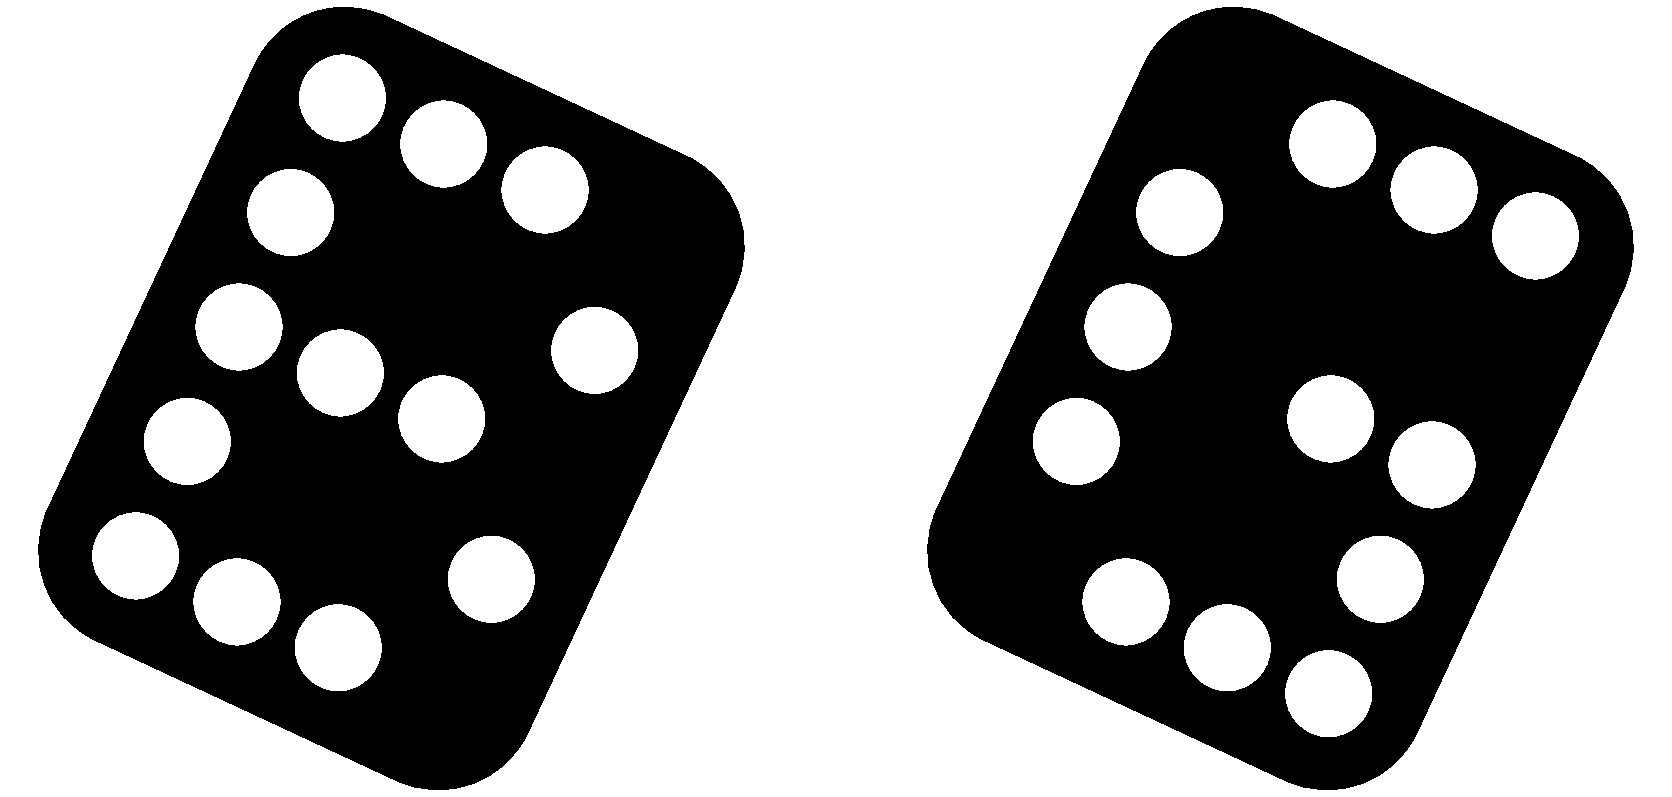
\includegraphics[height=30pt]{img/gaspedale/1.pdf}}}
	\newcommand{\pedaleRealistisch}{\raisebox{-.5ex}{
\includegraphics[height=30pt]{img/gaspedale/2.pdf}}}
	\newcommand{\tacho}{\raisebox{-.5ex}{
\includegraphics[height=30pt]{img/gaspedale/3.pdf}}}
	\newcommand{\autoPfeil}{\raisebox{-.5ex}{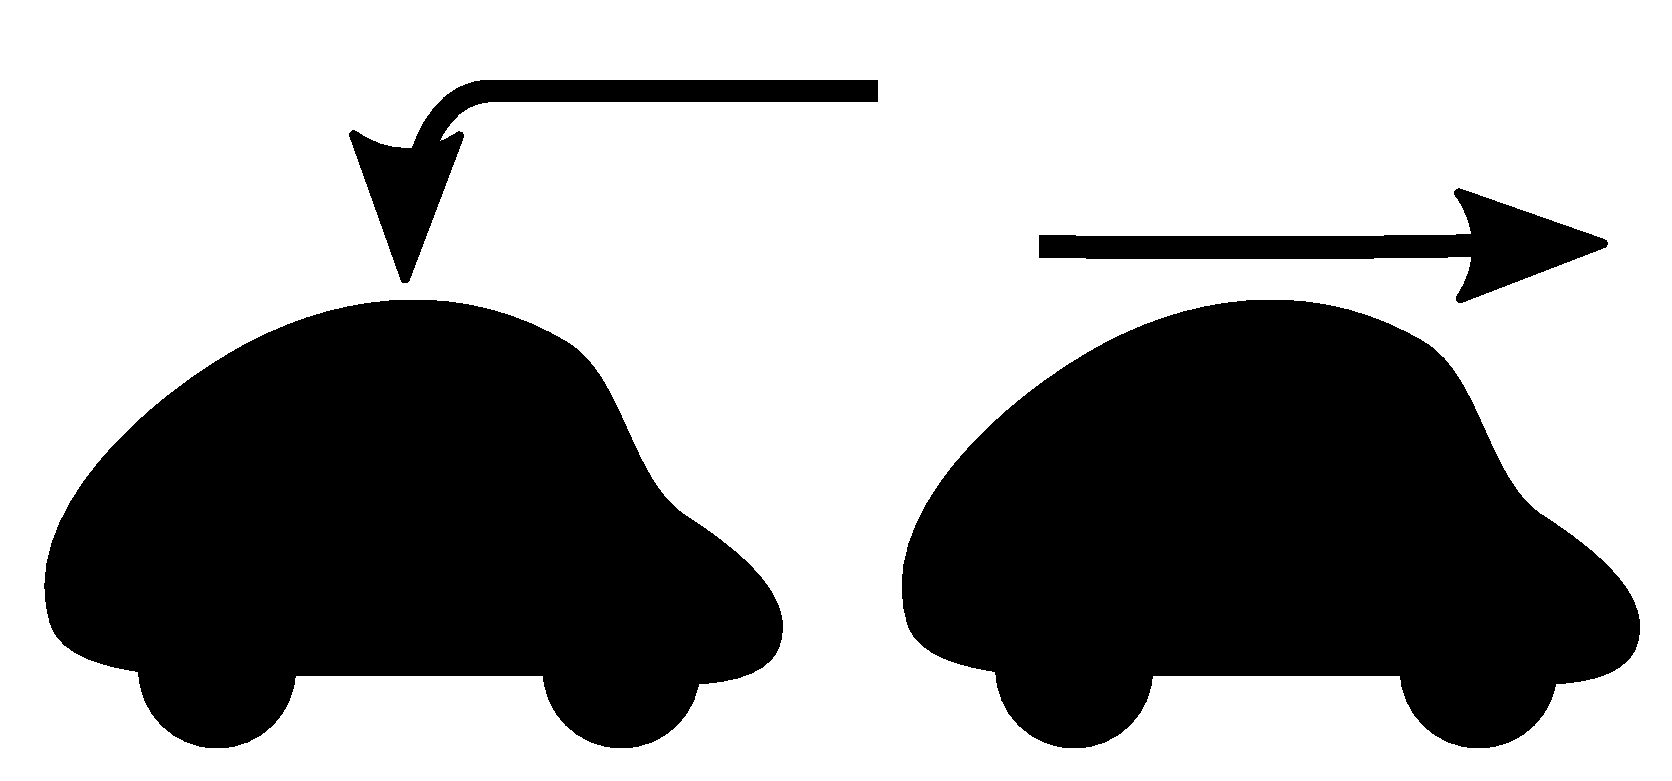
\includegraphics[height=30pt]{img/gaspedale/4.pdf}}}
	\newcommand{\symbolbild}{\raisebox{-.5ex}{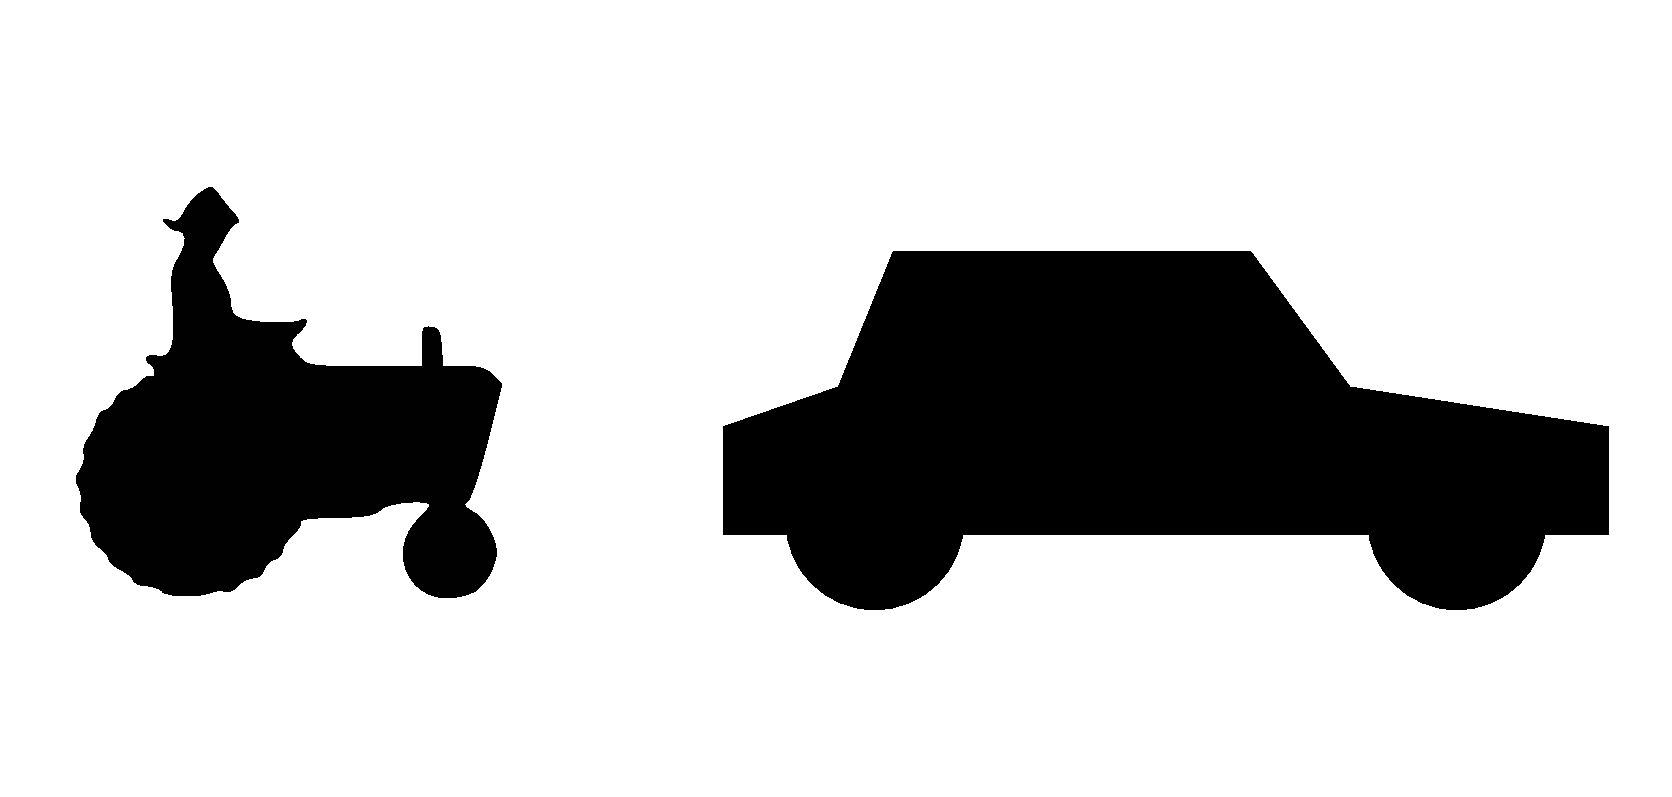
\includegraphics[height=30pt]{img/gaspedale/5.pdf}}}

	\begin{longtable}{cp{3.9cm}p{3.9cm}p{3.9cm}}%
		\toprule \endhead%
		\bottomrule \caption{Evolution der Pedale}\label{gasevo-tabelle} \endlastfoot%
			 & Beschreibung & Vorteile & Nachteile \\ \midrule
			\pedaleSchrift 		& Beschriftete Pedale werden in vielen Rennspielen verwendet. Dabei sind die Pedale mit \enquote{G} für Gas und \enquote{B} für Bremsen beschriftet. & Für deutschsprachige Spieler ist diese Einteilung einfach verständlich. & Im Rahmen der multilingualen Verwendbarkeit kann eine solche Beschriftung zu Missverständnissen führen. \\%
			\symbolbild 		& Eine weitere Möglichkeit ist die Verwendung von Symbolbildern. Dabei soll ein Symbol langsames Fahren und das andere schnelles Fahren symbolisieren. & Die Assoziation mit schnell und langsam ist sehr einfach. Die Symbole sind auch für Kinder sehr leicht verständlich. & Die Symbolbilder können nicht direkt als Schaltflächen erkannt werden. Eine Verwechslung mit beispielsweise einem Fahrzeugwechsel ist möglich und kann für Verwirrung sorgen.  \\%
			\autoPfeil 			&  Die Fahrzeuge werden mit entsprechenden erklärenden Pfeilen ausgestattet. Ein Pfeil zeigt auf das Fahrzeug selbst, was einen Stillstand symbolisiert. Der zweite Pfeil zeigt vom Fahrzeug weg, was eine Beschleunigung symbolisieren soll. & Durch die Verwendung des gleichen Fahrzeugs ist eine Assoziation mit einem Fahrzeugwechsel ausgeschlossen. & Die Bedeutung der jeweiligen Pfeile ist nicht eindeutig. Ein großer Interpretationsspielraum kann sehr leicht Missverständnisse hervorrufen. \\%
			\tacho 				& Zur Symbolisierung für schnelles und langsames Fahren werden Tachos mit unterschiedlichen Nadelausschlägen verwendet. Ein voll ausgeschlagener Tacho bedeutet dabei schnelles Fahren. & Da keine irritierenden Pfeile verwendet werden, sinkt die Gefahr eines Missverständnisses. Da ebenso kein Fahrzeug symbolisiert wird, kann auch jegliches Missverständnis in dieser Richtung vermieden werden. & Tachos sind leicht verwechselbar mit einer Benzinanzeige oder einer reinen Geschwindigkeitsanzeige. Usertests haben gezeigt, dass Spieler nicht intuitiv auf die Tachos drücken. \\%
			\pedaleRealistisch 	& Das finale Design geht zurück zu den Pedalen, verzichtet jedoch auf die Beschriftung. Zur besseren Unterscheidbarkeit werden unterschiedliche Designs für die jeweiligen Pedale gewählt. Dabei orientieren sich die Pedale an Pedalen von realen Fahrzeugen. & Die Pedale sind einfach als Schaltflächen erkennbar, durch das Verzichten auf Beschriftung sind die Pedale multilingual einsetzbar. Durch die Orientierung an realen Pedalen ist eine Assoziation mit diesen gegeben. & Der Spieler erkennt zwar nicht auf den ersten Blick, welche Funktion die Schaltflächen haben, kann dies jedoch über \enquote{Ausprobieren} testen. \\%
	\end{longtable}
	Der letzte Punkt im Bereich des UI Designs befasst sich mit der grundsätzlichen Positionierung der Schaltflächen und Icons. Wie in <TODO: Verlinkung zum Konzept> bereits erwähnt, soll das Spiel auf mobilen Endgeräten im Querformat gespielt und mit zwei Händen bedient werden. Da die wichtigsten Steuerelemente der Joystick sowie die Pedale sind, werden diese in den unteren Ecken zur Bedienung mit beiden Daumen positioniert. Die Schaltflächen für Pause und Zurücksetzen sind in den oberen Ecken positioniert, um eine versehentliche Betätigung durch den Spieler zu verhindern.
	\figur{Positionierung-UI.png}{\label{ssec:ui-design}User Interface mit geöffnetem Menü}
	Die Abbildung \ref{ssec:ui-design} zeigt das User Interface, während das Menü geöffnet ist. Die Menü-Schaltflächen für \enquote{Spiel fortsetzen / Spiel starten}, \enquote{Optionsmenü öffnen} sowie \enquote{Zum Hauptmenü zurückkehren} sind an der Mitte des Bildschirms orientiert.
	\figur{Positionierung-UI-2.png}{\label{ssec:ui-design2}User Interface während des Rennens}
	Während des Spiels entspricht das User Interface der Abbildung \ref{ssec:ui-design2}. An Stelle der Schaltflächen des Menüs befinden sich am oberen Bildschirmrand nun eine Zeitanzeige, sowie eine Minikarte. Die Minikarte stellt den Streckenverlauf leicht transparent dar und zeigt die Position und Rotation des Fahrzeugs mittels eines roten Pfeils an. Die Zeitanzeige ist als Zeitstrahl dargestellt. Dabei sinkt die Größe des gelben Anteils des Zeitstrahls. Ist kein gelber Anteil mehr vorhanden, so ist die Zeit für das Rennen vollständig abgelaufen.

	\subsubsection{Umsetzung der Steuerung}
	Die Steuerung des Fahrzeugs ergibt sich aus dem Zusammenspiel vieler Komponenten und Code-Bestandteile, welche über mehrere Skripte verteilt sind. In diesem Kapitel werden aus diesem Grund lediglich die wichtigsten Kernaspekte der Steuerung erläutert. Der Prozess der Steuerung läuft dabei in mehreren Schritten ab:
	\begin{enumerate}
		\item{ Das \enquote{CarUserControl} Skript entscheidet, ob das Fahrzeug fahren darf. }
		\item{ Falls ja erteilt das Skript dem \enquote{CarController} Skript den Befehl zur Bewegung }
		\item{ Im CarController wird die Ausrichtung des Joysticks ausgelesen. }
		\item{ Im CarController wird berechnet, um wie viel Grad das Fahrzeug drehen muss, um den gewünschten Winkel zu erhalten. }
		\item{ Die Räder werden im entsprechenden Winkel gedreht und das Fahrzeug bewegt sich in diese Richtung. }
	\end{enumerate}
	Im Folgenden sollen diese Schritte genauer analysiert werden. Dabei wird die Nummerierung aus der Aufzählung als Referenz verwendet.
	\begin{lstlisting}
private void FixedUpdate(){
[...]
//Überprüfe ob sich das Fahrzeug bewegen darf
  if (car.canMove){
    //Übermittle Befehl zur Bewegung
    m_Car.Move([...]]);
  }
}
	\end{lstlisting}
	Im CarUserControl Skripts aus Schritt 1 wird regelmäßig die FixedUpdate() Methode ausgeführt. Regelmäßig bedeutet in diesem Fall eine Ausführung für jedes auf dem Bildschirm angezeigte Bild. Ob das Fahrzeug fahren darf, ist vom derzeitigen Status des \enquote{RaceController} Skripts abhängig. Der RaceController ist die Haupt-Kontrollinstanz für jedes gefahrene Rennen. Befindet sich der Spieler im Hauptmenü, so darf das Fahrzeug beispielsweise nicht fahren. In dem Moment, in welchem der Countdown vor einem Rennen abläuft, wird die Variable \enquote{canMove} auf \emph{true} gesetzt und das Fahrzeug darf losfahren. In diesem Moment übergibt die CarUserControl den Befehl zur Bewegung an den CarController.

	\begin{lstlisting}
public void Move([...]){
[...]
//Berechne Richtungsvektor des Joysticks
Vector3 direction =
  CrossPlatform.GetAxis("Vertical") * -Vector3.right
  + CrossPlatform.GetAxis("Horizontal") * Vector3.forward;
//Berechne den Drehwinkel zwischen aktueller Rotation des Fahrzeugs und der gewünschten Ausrichtung
Quaternion rotation = Quaternion.FromToRotation(
	(transform.rotation * Vector3.forward), direction);
	\end{lstlisting}

	Im nächsten Schritt wertet der CarController die Eingaben des Joysticks aus. Dazu greift er auf die Informationen des CrossPlatformInputManagers (im Codebeispiel als CrossPlatform abgekürzt) zurück. Dieser liefert Informationen über die horizontale und vertikale Ausrichtung des Joysticks. Dies sind generell Werte zwischen $-1$ und $1$. Durch Vektormultiplikationen mit den beiden Einheitsvektoren (x- und y-Richtung) entsteht ein Richtungsvektor. Dieser Richtungsvektor ist zweidimensional (bzw. der z-Wert ist immer $0$) und stellt die Zugrichtung des Joysticks dar.
	Aus der derzeitigen Ausrichtung des Fahrzeugs und dem zuvor errechneten Richtungsvektor kann eine Quaternion errechnet werden. Eine Quaternion beschreibt eine Bewegung eines Objekts. Die errechnete Quaternion beschreibt somit eine Rotation des Objekts von der derzeitigen Ausrichtung hin zur gewünschten Ausrichtung.

	\begin{lstlisting}
//Berechne Drehwinkel der Vorderräder
bool forwards = true;
steerAngle = rotation.eulerAngles.y;
if (180 - Mathf.Abs(steerAngle - 180) > m_MaximumSteerAngle){
  //Überprüfe, ob Fahrzeug rückwärts fährt
  if (steerAngle > 135 && steerAngle < 225){
	forwards = false;
	steerAngle = 360 - steerAngle;
	//Drehe Hinterräder um 180 Grad
	wheelCol[2].steerAngle = wheelCol[3].steerAngle = 180;
  } else {
    if (steerAngle >= 225){
	  steerAngle = 360 -m_MaximumSteerAngle;
    } else {
  	  steerAngle = m_MaximumSteerAngle;
    }
  wheelCol[2].steerAngle = wheelCol[3].steerAngle = 0;
  }
}
	\end{lstlisting}

	Im letzten Schritt müssen die Räder des Fahrzeugs entsprechend ausgerichtet werden. Dabei wird zunächst aus der Rotation ein Drehwinkel berechnet. Über die Fallunterscheidung aus dem Codebeispiel oben wird bestimmt, ob der Joystick entgegen der Fahrzeugausrichtung bewegt wird. Eine Bewegung entgegen der Ausrichtung des Fahrzeugs wird dabei als \enquote{Befehl zum Rückwärtsfahren} interpretiert. Um eine realistische Kurvenbahn zu erhalten, wird der Drehwinkel der Räder auf einen Bereich zwischen -45° und +45° begrenzt. Ein Bewegen des Joysticks außerhalb dieses Bereichs setzt den Winkel auf das jeweilige Maximum fest. So wird beispielsweise -60° in -45° umgewandelt. Somit ist gewährleistet, dass das Fahrzeug konstante Kurven fährt und das Angleichen der Fahrtrichtung an die Position des Joysticks nicht zu ruckartig geschieht. Das Verhalten der Räder bei Einschlagen des Rückwärtsgangs stellt eine Besonderheit dar. Die Räder sind mit einer Rotationsrichtung versehen, welche nicht einfach invertiert werden kann. Aus diesem Grund müssen alle Räder vollständig invertiert werden, wenn der Nutzer das Fahrzeug rückwärts steuern möchte. Die Hinterräder werden in diesem Fall exakt um 180° gedreht, die Vorderräder werden erst auf Basis des Lenkwinkels ausgerichtet und dann um 180° rotiert. Sobald die Fahrtrichtung wieder auf vorwärts wechselt, werden alle Räder erneut invertiert.

	Zur Realisierung der Beschleunigung ist eine Betrachtung des Rückwärtsgangs somit nicht nötig. Für die Beschleunigung wird eine zusätzliche Achse \enquote{Acceleration} entwickelt, welche mit dem Gaspedal verknüpft wird. Ein Betätigen des Gaspedals setzt den Wert der Achse auf 1, im generellen Fall beträgt der Wert 0. Das Bremspedal ist auf sehr ähnliche Weise definiert, ein Betätigen des Pedals setzt einen Wert \enquote{Bremskraft}, welcher ebenso wie die Beschleunigung in die generelle Bewegungsfunktion des Fahrzeugs eingebunden ist.


	\subsubsection{Physik}
	Im Rahmen dieser Arbeit wird auf die Entwicklung einer eigenen Physiksimulation verzichtet. Für die Implementierung der physikalisch interagierbaren Objekte wird auf die Grundfunktionen der Unity Engine zurückgegriffen. So können Objekte mit sogenannten \enquote{Physical Materials} versehen werden. Über diese Physical Materials können Objekte beispielsweise eine gewisse Elastizität erreichen oder wie Gummibälle von Gegenständen und Wänden abprallen. Über die Physical Materials wird versucht, die Reaktion der Objekte der Realität anzupassen. Die Leitkegel erhalten dabei einen höheren \enquote{Bouncyness} Wert als die Fässer, was dazu führt, das Leitkegel eher vom Fahrzeug abprallen, wohingegen Fässer eher vom Fahrzeug verschoben werden. Dieses Verhalten wird durch den erhöhten Gewichtswert der Fässer verstärkt, welcher dazu führt, dass die Fässer das Fahrzeug stärker abbremsen.

	\subsubsection{Verlangsamung des Fahrzeugs}
	\begin{lstlisting}
public void adjustTopSpeed()
{
float changeFactor = -Mathf.Cos(m_Topspeed/80 - 0.2f)*1.5f+1.6f;
if (isSlow){
    m_Topspeed = Mathf.Max(m_Topspeed - changeFactor * 1.3f, m_TopspeedSlow);
}else{
    m_Topspeed = Mathf.Min(m_Topspeed + changeFactor, m_TopspeedNormal);
}
}
    \end{lstlisting}
    Das Codebeispiel oben zeigt die beiden mathematischen Funktionen, welche für die Verlangsamung des Fahrzeugs verantwortlich sind. Der Methodenaufruf der adjustTopSpeed() Methode geschieht immer dann, wenn das Fahrzeug eine Zone betritt oder verlässt, welche die Geschwindigkeit manipuliert. Beim Betreten einer so genannten \enquote{SlowDown}-Zone wird die Variable \enquote{isSlow} auf \enquote{true} gesetzt. Daraufhin wird die Höchstgeschwindigkeit des Fahrzeugs kontinuierlich reduziert, bis die festgesetzte Geschwindigkeit erreicht ist. Verlässt das Fahrzeug die SlowDown-Zone wieder, so wird isSlow auf \enquote{false} gesetzt und die Höchstgeschwindigkeit des Fahrzeugs wird kontinuierlich erhöht, bis die ursprüngliche Höchstgeschwindigkeit erreicht ist.

	\subsubsection{Erkennung einer Frontalkollision}
	Um die Erkennung einer Frontalkollision zu ermöglichen, wird das Fahrzeug mit zwei Hilfs-Punkten ausgestattet. Diese Punkte sind jeweils mittig des Fahrzeugs positioniert, wobei einer der Punkte am vorderen Ende des Fahrzeugs und der zweite Punkt am Heck positioniert ist.
	\begin{lstlisting}
private void OnCollisionEnter(Collision collision){
Vector3 localAverageVorn = frontColliderHelper.transform.InverseTransformPoint(collision.contacts[0].point);
float distVorn = Vector3.Distance(localAverageVorn, new Vector3(0, 0, 0));
Vector3 localAverageBack = backColliderHelper.transform.InverseTransformPoint(collision.contacts[0].point);
float distBack = Vector3.Distance(localAverageBack, new Vector3(0, 0, 0));
if (distVorn <= 0.8 || distBack <= 0.8)
{
float speed = collision.relativeVelocity.magnitude;
float volume = Mathf.Pow(Mathf.Clamp(speed/10, 0f, 1f), 3);
GetComponent<NewGameAudio>().playCrashSound(volume);
}
}
\end{lstlisting}
	Das gezeigte Skript ist eine Komponente des Fahrzeugs. Im Moment der Kollision werden alle relevanten Daten über das kollidierte Objekt in einem Kollisions-Objekt gespeichert. Aus der Kollision können die Kontaktpunkte der beiden Objekte ausgelesen werden. Im nächsten Schritt wird die Durchschnittsposition aller Kontaktpunkte (also der mittlere aller Punkte) mit beiden eingangs erwähnten Hilfs-Punkten vergleichen. Dabei werden die derzeitigen Weltkoordinaten (Positionierung relativ zum Levelmittelpunkt) beider Punkte verwendet und die Distanz dieser beiden Punkte errechnet. Ist einer der beiden errechnet Werte (\enquote{distVorn} oder \enquote{distBack}) kleiner oder gleich 0.8, so wird von einer Frontalkollision ausgegangen. Der Abstand von 0.8 ist so gewählt, dass die äußeren Ecken des Fahrzeugs noch als Frontalkollision erkannt werden, seitlich versetzte Kollisionen jedoch nicht. Somit kann für beide Fälle ein anderer Sound abgespielt werden. Im Fall einer Frontalkollision wird ein Aufprall-Sound abgespielt, bei einer seitlichen Kollision ertönt ein \enquote{Kratzen}.
	Die Lautstärke des abgespielten Tons errechnet sich dabei aus der Geschwindigkeit des Fahrzeugs zum Zeitpunkt der Kollision. Je schneller das Fahrzeug mit einem Objekt kollidiert, desto lauter wird der Sound abgespielt.

	\subsubsection{Speicherung der Spielstände\label{speicherung}}
	Für die Speicherung der Spielstände stehen zwei Möglichkeiten zur Verfügung. Zum einen kann eine Datenbank eingebunden werden, welche alle relevanten Daten speichert, zum anderen kann eine Datei erstellt werden, welche mittels serialisierbaren Feldern Informationen über den Spielfortschritt bereitstellt. Serialisierbarkeit bedeutet, dass die Werte eines Feldes codiert und auch aus dem Code reproduziert werden können.
	Da keine großen Datenmengen zu erwarten sind, wird eine Datei im \enquote{.bin Format} verwendet.
	Die im Nutzerverzeichnis des Endgeräts befindliche \enquote{GameData.bin} enthält Informationen über die bereits gewonnenen Rennen, über freigeschaltete Gegenstände aus dem Shop, über die Anzahl an Münzen, die der Nutzer besitzt, sowie die aus dem Shop ausgerüsteten Gegenstände. Dadurch ist gewährleistet, dass der Nutzer das Spiel bei einem Neustart im gleichen Zustand vorfindet, wie es verlassen wurde.
	Alle genannten Attribute sind über sogenannte [SerializeField] Attribute definiert, was eine Speicherung im Textformat ermöglicht. Über den Aufruf \enquote{GameData.GetInstance()} kann an jeder beliebigen Stelle des Programmcodes auf die gespeicherten Werte zugegriffen werden. Somit ist eine Anwendungsweite Synchronisation gewährleistet.

	\subsubsection{Performance und Dateigröße}
	Ein wichtiger Schritt der Entwicklung des Spiels ist die Performance der Anwendung. Durch die Vorgaben der Aufgabenstellung soll das Spiel auch für Kinder der ärmeren Bevölkerungsschichten zugänglich sein. Kinder, die diesen Schichten angehören, besitzen häufig keine sehr guten mobilen Geräte. Somit rückt die Performance in den Vordergrund.
	Vor der Optimierung der Anwendung ist diese auf einem \emph{HTC ONE M8} gerade so spielbar. Die Anwendung ruckelt leicht, ein erfolgreiches Abschließen der Level ist jedoch ohne weiteres möglich. Auf dem zweiten Testgerät, einem \emph{Samsung Galaxy S2} sowie auf dem \emph{Fairphone 2} ist die Anwendung unspielbar und springt langsam von einem Standbild zum nächsten.
	Hinzu kommt, dass die Anwendung in diesem Status der Entwicklung zu viel Speicherplatz einnimmt. Vor der Optimierung beträgt die Größe der APK-Installationsdatei ca $100$ MB, das installierte Spiel nimmt $280$ MB ein.

	Für die Optimierung der Performance und der Dateigröße werden folgende Schritte definiert:
	\begin{itemize}
	\item{ Reduzierung der Dateigröße durch höhere Kompression der Texturen.}
	\item{ Verbesserung der Performance durch geringere Qualitätseinstellungen für Texturen und 3D Modelle.}
	\item{ Optimierung der Performance durch entfernen einiger Elemente aus den Leveln.}
	\item{ Reduzierung der Dateigröße durch geringere Standardgröße aller 3D Objekte.}
	\end{itemize}

	Nach der Durchführung der vier genannten Schritte ist eine deutliche Optimierung sichtbar. Die Dateigröße der APK-Installationsdatei ist auf etwa $70$ MB gesunken, die Größe des installierten Spiels auf dem Endgerät beträgt lediglich noch $128$ MB.
	Auf dem \emph{HTC ONE M8} läuft die Anwendung merklich flüssiger, die leichten Ruckler sind kaum erkennbar. Auf dem \emph{Samsung Galaxy S2} konnte die Anwendung leider nicht flüssig ausgeführt werden. Die Bildrate ist durch die Optimierung merklich gestiegen, jedoch ist ein gut spielbarer Status nicht erreicht. Auf dem \emph{Fairphone 2} konnte die optimierte Anwendung bis zum aktuellen Zeitpunkt nicht erneut getestet werden.

	Die Verteilung der einzelnen Optimierungsschritte sieht dabei wie folgt aus:
	Die Reduzierung der Standardgröße aller 3D Objekt hat leider nicht den gewünschten Effekt erzielt. Die endgültige Dateigröße hat sich durch diesen Schritt um lediglich $2$ MB verkleinert. Die höhere Kompression der Texturen hatte im Rahmen der Optimierung den größten Effekt. Die Größe aller Texturen konnte von insgesamt rund $240$ MB auf $20$ MB verringert werden. Diese Werte sind nicht direkt im Gesamtergebnis erkennbar, da die Texturen im Laufe des Build-Prozesses erneut komprimiert werden.
	Im Rahmen der Performanceoptimierung konnte der größte Erfolg durch das Entfernen einiger Elemente aus den Leveln erzielt werden. Die geringeren Qualitätseinstellungen für Texturen und Modelle verändern hierbei lediglich die Optik, verändern jedoch die Performance nur minimal.

\subsection{Struktur und Aufbau}
Wie im vorherigen Kapitel bereits erwähnt, werden Programmfunktionen in Unity grundsätzlich über Skripte realisiert. Diese Skripte sind in den meisten Fällen unabhängig voneinander. Das Zusammenfügen der Komponenten wird in diesem Fall von der Unity Engine übernommen. Von einer Darstellung aller internen Komponenten der Engine wird an dieser Stelle abgesehen, da während der Entwicklung des Spiels kein Einfluss auf diese internen Verknüpfungen genommen werden kann. Eine Darstellung der einzelnen Skripte zeigt lediglich voneinander unabhängige Dateien. Dies erzeugt für die Arbeit keinen Mehrwert, daher wird darauf verzichtet. Allgemein zusammengefasst lässt sich ableiten: Die Unity Engine steht in der Mitte eines Diagramms, viele Skripte sind in Form einer Wolke um die Engine verteilt, stehen jedoch nicht in Verbindung zueinander.
Bei der Implementierung des Spiels wurde keine Datenbank verwendet. Die Datenspeicherung geschieht wie in \ref{speicherung} bereits erwähnt über die Datei \enquote{GameData.bin}.

\subsection{Integration in Lernplattform}
	Die Integration in die Lernplattform von Incekara und Wolske\footcite{lernplattform} konnte nicht umgesetzt werden. Die Möglichkeiten des Spiels verschiedene Lernstandards gleichzeitig zu implementieren sind nicht in der Plattform vorgesehen und es müsste eine Schnittstelle implementiert werden.
	Eine Möglichkeit diese Schnittstelle umzusetzen wurde ausgearbeitet aber schlussendlich nicht verwendet.
	\subsubsection*{Beschreibung Schnittstelle}
		Für die Kommunikation zwischen Anwendungen auf Android ist die Verwendung von AIDL\footcite{android-interfaces} oder ähnlichem nötig.\footnote{Weitere Möglichkeiten werden auf der zitieren Seite genannt.}
		Ein unterstütztes Lernspiel bietet zwei Schnittstellen:
		\begin{description}
			\item[Lernstandards auflisten]{
				Gibt eine Liste der unterstützten Standards zurück.
			}
			\item[Mit Standard $X$ starten]{
				Startet das Spiel mit dem ausgewählten Standard.
			}
		\end{description}
		Für die Lernplattform reicht es aus die Standards beim Starten für alle Spiele zu sammeln und wenn vom Spieler gewünscht diese mit dem Passendem Standard starten.
